\documentclass{article}
\usepackage[spanish]{babel}
\usepackage[onehalfspacing]{setspace}
\usepackage[utf8]{inputenc}
\usepackage{amsmath}
\usepackage{amssymb}
\usepackage{verbatim}
\usepackage{graphicx}
\usepackage{listings}
\usepackage{fullpage}
\usepackage{color}
\usepackage{fancyvrb}
\usepackage{hyperref}
\usepackage{appendix}
\hypersetup{%
	pdfborder = {0 0 0}
}

\definecolor{mygreen}{rgb}{0,0.6,0}
\definecolor{mygray}{rgb}{0.5,0.5,0.5}
\definecolor{mymauve}{rgb}{0.58,0,0.82}

\lstset{ %
	backgroundcolor=\color{white},   % choose the background color; you must add \usepackage{color} or \usepackage{xcolor}
	basicstyle=\footnotesize,        % the size of the fonts that are used for the code
	breakatwhitespace=false,         % sets if automatic breaks should only happen at whitespace
	breaklines=true,                 % sets automatic line breaking
	captionpos=b,                    % sets the caption-position to bottom
	commentstyle=\color{mygreen},    % comment style
	frame=single,                    % adds a frame around the code
	keepspaces=true,                 % keeps spaces in text, useful for keeping indentation of code (possibly needs columns=flexible)
	numbers=left,                    % where to put the line-numbers; possible values are (none, left, right)
	numbersep=5pt,                   % how far the line-numbers are from the code
	numberstyle=\tiny\color{mygray}, % the style that is used for the line-numbers
	rulecolor=\color{black},         % if not set, the frame-color may be changed on line-breaks within not-black text (e.g. comments (green here))
	showspaces=false,                % show spaces everywhere adding particular underscores; it overrides 'showstringspaces'
	showstringspaces=false,          % underline spaces within strings only
	showtabs=false,                  % show tabs within strings adding particular underscores
	stepnumber=1,                    % the step between two line-numbers. If it's 1, each line will be numbered
	stringstyle=\color{mymauve},     % string literal style
	tabsize=4,
	title=\lstname                   % show the filename of files included with \lstinputlisting; also try caption instead of title
}


\author{José Luis Cánovas Sánchez\\joseluis.canovas2@um.es\\48636907A}
\title{ARQUITECTURAS DE REDES AVANZADAS\\PRÁCTICA 2\\Balanceo de Carga con SDN\\ ENERO 2015}
\date{}
\begin{document}
\maketitle

\tableofcontents

\section{Topología mininet}

La topología implementada en mininet corresponde, como se puede ver en la \autoref{fig:topology} a dos switch conectados al controlador, 6 máquinas cliente y 4 servidores.


\begin{figure}[!h]
	\centering
	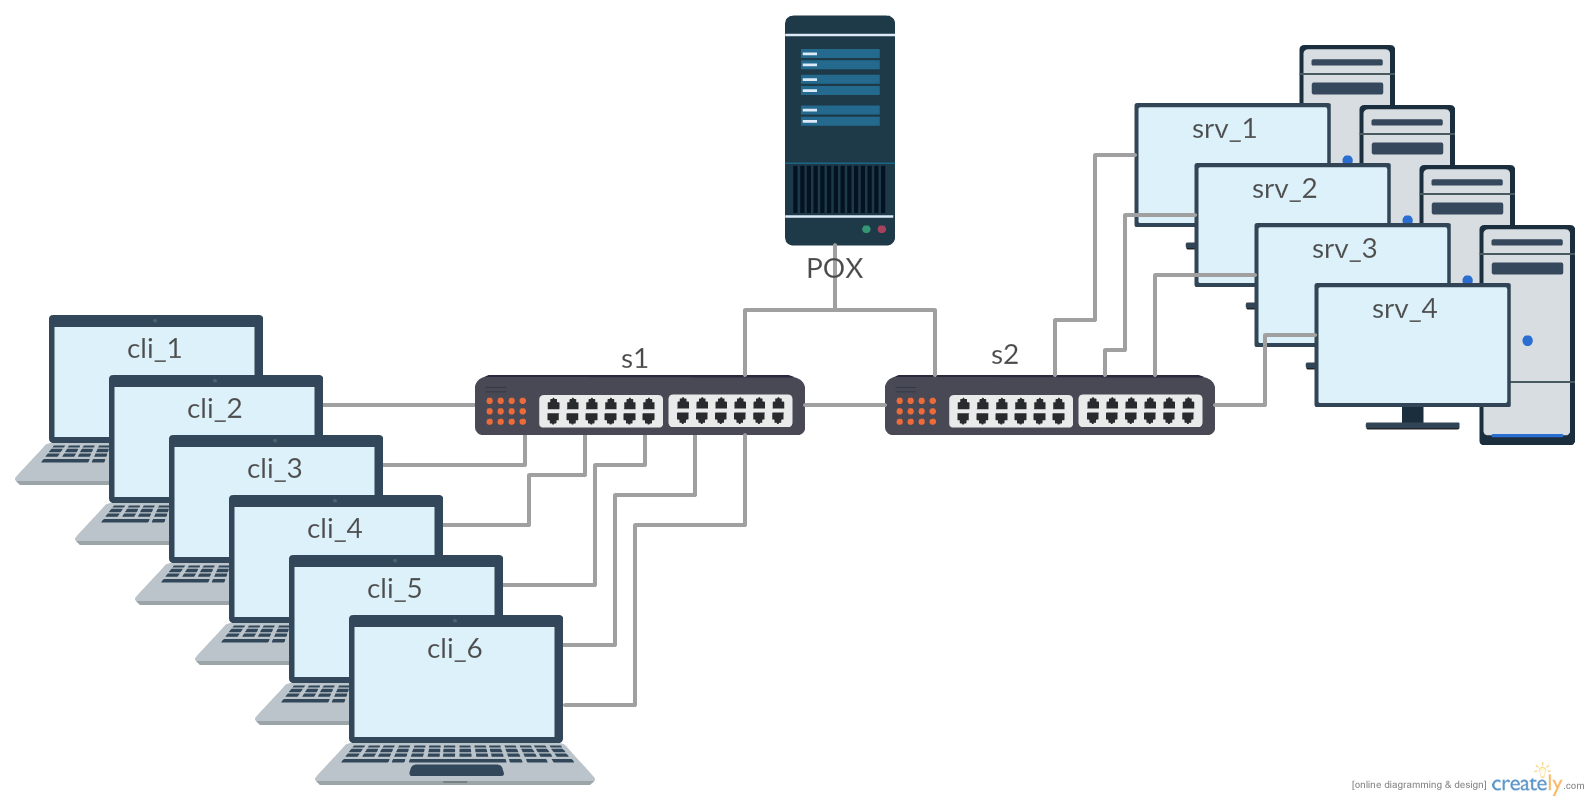
\includegraphics[scale=0.29]{images/topology.png}
	\caption{Topología}
	\label{fig:topology}
\end{figure}

\hfill

El código en python que define a la topología es el siguiente. Para facilitar las pruebas, a los servidores se les da una dirección MAC prefijada en el método \textit{addHost}, y a las conexiones con el switch `s2'  siempre se indican a qué puerto conectar, con el parámetro \textit{port2} del método \textit{addLink}.

\begin{lstlisting}[language=Python]
# -*- coding: utf-8 -*-

from mininet.topo import Topo

class MyTopo (Topo):

    def __init__ (self):
        Topo.__init__( self )

        # Add switches
        sw_clients = self.addSwitch('s1')
        sw_servers = self.addSwitch('s2')

        # Add clients
        c1 = self.addHost('cli_1')
        c2 = self.addHost('cli_2')
        c3 = self.addHost('cli_3')
        c4 = self.addHost('cli_4')
        c5 = self.addHost('cli_5')
        c6 = self.addHost('cli_6')

        # Add servers
        s1 = self.addHost('srv_1', ip='10.0.0.101', mac='00:00:00:00:01:01')
        s2 = self.addHost('srv_2', ip='10.0.0.102', mac='00:00:00:00:01:02')
        s3 = self.addHost('srv_3', ip='10.0.0.103', mac='00:00:00:00:01:03')
        s4 = self.addHost('srv_4', ip='10.0.0.104', mac='00:00:00:00:01:04')

        # Add links
        self.addLink(sw_clients, sw_servers, port2=1)

        self.addLink(c1, sw_clients)
        self.addLink(c2, sw_clients)
        self.addLink(c3, sw_clients)
        self.addLink(c4, sw_clients)
        self.addLink(c5, sw_clients)
        self.addLink(c6, sw_clients)

        self.addLink(s1, sw_servers, port2=2)
        self.addLink(s2, sw_servers, port2=3)
        self.addLink(s3, sw_servers, port2=4)
        self.addLink(s4, sw_servers, port2=5)


topos = {'mytopo': lambda: MyTopo()}
\end{lstlisting}

\section{Controlador POX con l2\_learning}

Realizamos un test básico de la topología anterior usando el fichero \textit{l2\_learning} que proporciona POX.

La salida por pantalla de mininet durante la prueba es la siguiente:

\begin{Verbatim}[frame=single]
$sudo mn --custom topo.py --topo mytopo --controller remote --test pingall
	*** Creating network
	*** Adding controller
	*** Adding hosts:
	cli_1 cli_2 cli_3 cli_4 cli_5 cli_6 srv_1 srv_2 srv_3 srv_4
	*** Adding switches:
	s1 s2
	*** Adding links:
	(cli_1, s1) (cli_2, s1) (cli_3, s1) (cli_4, s1) (cli_5, s1)
	 (cli_6, s1) (s1, s2) (srv_1, s2) (srv_2, s2) (srv_3, s2) (srv_4, s2)
	*** Configuring hosts
	cli_1 cli_2 cli_3 cli_4 cli_5 cli_6 srv_1 srv_2 srv_3 srv_4
	*** Starting controller
	c0
	*** Starting 2 switches
	s1 s2 ...
	*** Waiting for switches to connect
	s1 s2
	*** Ping: testing ping reachability
	cli_1 -> cli_2 cli_3 cli_4 cli_5 cli_6 srv_1 srv_2 srv_3 srv_4
	cli_2 -> cli_1 cli_3 cli_4 cli_5 cli_6 srv_1 srv_2 srv_3 srv_4
	cli_3 -> cli_1 cli_2 cli_4 cli_5 cli_6 srv_1 srv_2 srv_3 srv_4
	cli_4 -> cli_1 cli_2 cli_3 cli_5 cli_6 srv_1 srv_2 srv_3 srv_4
	cli_5 -> cli_1 cli_2 cli_3 cli_4 cli_6 srv_1 srv_2 srv_3 srv_4
	cli_6 -> cli_1 cli_2 cli_3 cli_4 cli_5 srv_1 srv_2 srv_3 srv_4
	srv_1 -> cli_1 cli_2 cli_3 cli_4 cli_5 cli_6 srv_2 srv_3 srv_4
	srv_2 -> cli_1 cli_2 cli_3 cli_4 cli_5 cli_6 srv_1 srv_3 srv_4
	srv_3 -> cli_1 cli_2 cli_3 cli_4 cli_5 cli_6 srv_1 srv_2 srv_4
	srv_4 -> cli_1 cli_2 cli_3 cli_4 cli_5 cli_6 srv_1 srv_2 srv_3
	*** Results: 0\% dropped (90/90 received)
	*** Stopping 1 controllers
	c0
	*** Stopping 11 links
	...........
	*** Stopping 2 switches
	s1 s2
	*** Stopping 10 hosts
	cli_1 cli_2 cli_3 cli_4 cli_5 cli_6 srv_1 srv_2 srv_3 srv_4
	*** Done
	completed in 6.529 seconds
\end{Verbatim}

Todos los hosts (clientes y servidores) tienen conectividad entre ellos y ningún paquete ICMP se ha perdido. La topología de mininet es correcta y se conecta con el controlador POX.

\section{Construcción del balanceador de carga}

\subsection{Módulo de balanceo en POX}

Partimos del fichero \textit{l2\_learning.py} y añadimos las siguientes líneas de código en la clase LearningSwitch.

Las primeras líneas sirven para definir el método que por round-robin devuelve el siguiente puerto del switch s2 por el que balancear una nueva conexión a los servidores.

\begin{lstlisting}[language=Python]
class LearningSwitch (object):
	[...]
	 def __init__ (self, connection, transparent):
		[...]
		self.round_robin = 0
		self.max_srvs = 4
		self.frst_prt = 2

	def roundRobin(self):
		rr = (self.round_robin%self.max_srvs) + self.frst_prt
		self.round_robin+=1
		return rr
\end{lstlisting}


Estas líneas se añaden en \_handle\_PacketIn casi al inicio del método, después de aprender el puerto para la MAC del origen (añadiendo una entrada en \textit{macToPort}), y comprobamos que sea un mensaje del switch 2, que es el que debe balancear, que es un ARP REQUEST y que pregunta por la máquina con IP la de nuestros servidores balanceados.

En caso de ser un paquete que cumple todo lo anterior, creamos un mensaje para el switch s2 que añadirá a su tabla un nuevo flujo para todo paquete con MAC origen la del cliente que se envíe por el puerto del switch que indique el método del round-robin.

\begin{lstlisting}[language=Python]
def _handle_PacketIn (self, event):
	[...]
	# Round-Robin
	if ( dpid_to_str(event.dpid) == "00-00-00-00-00-02" and
                         packet.type == packet.ARP_TYPE and
                   packet.payload.opcode == arp.REQUEST and
                      packet.next.protodst == "10.0.0.101" ):
		msg = of.ofp_flow_mod()
		msg.match.dl_src = packet.src
		msg.actions.append(of.ofp_action_output(port = self.roundRobin()))
		#msg.idle_timeout = 10
		#msg.hard_timeout = 30
		msg.data = event.ofp
		self.connection.send(msg)
		return

	if packet.dst.is_multicast:
		flood() # 3a
	[...]
\end{lstlisting}


\subsection{Modificación topología}

A la topología de mininet el único cambio que hay que aplicarle es modificar las líneas 22 a 26, modificando la IP en \textit{addHost} por la 10.0.0.101, y que así sea única para todos los servidores.

\subsection{Ejecución y prueba de PING}

En el anexo al final de esta memoria se encuentra la salida por pantalla completa de las pruebas realizadas, y a continuación se muestra parte de las pruebas con ping aplicadas.

Para cada cliente se ejecuta la orden \textit{cli\_i ping -c 4 10.0.0.101}, 4 pings a la dirección de los servidores, que como vemos el primero tiene un retardo bastante considerable frente a los 3 siguientes, debido a que con el primero de todos el switch debe comunicarse con el controlador que se asigna el flujo para la MAC del cliente. Como el flujo se guarda en el switch, se aplica instantáneamente con los siguientes mensajes.

Además se realiza un \textit{pingall} que muestra que los 6 clientes alcanzan, como en l2\_learning a todas las máquinas. Sin embargo, los servidores, a pesar de poder hacer ping al resto de servidores, sólo reciben respuesta de uno o dos clientes, pues las respuestas tienen MAC origen la del cliente, y se reenvían al puerto asignado por round-robin en los pings anteriores. Por ejemplo, a los clientes 1 y 5 se les asignó, de los 4 servidores, el \textit{srv\_1}.

\hfill

\begin{Verbatim}
mininet> cli_6 ping -c 4 10.0.0.101
PING 10.0.0.101 (10.0.0.101) 56(84) bytes of data.
64 bytes from 10.0.0.101: icmp_seq=1 ttl=64 time=38.9 ms
64 bytes from 10.0.0.101: icmp_seq=2 ttl=64 time=0.448 ms
64 bytes from 10.0.0.101: icmp_seq=3 ttl=64 time=0.597 ms
64 bytes from 10.0.0.101: icmp_seq=4 ttl=64 time=0.352 ms

--- 10.0.0.101 ping statistics ---
4 packets transmitted, 4 received, 0% packet loss, time 3006ms
rtt min/avg/max/mdev = 0.352/10.082/38.933/16.657 ms
mininet> pingall
*** Ping: testing ping reachability
cli_1 -> cli_2 cli_3 cli_4 cli_5 cli_6 srv_1 srv_2 srv_3 srv_4
cli_2 -> cli_1 cli_3 cli_4 cli_5 cli_6 srv_1 srv_2 srv_3 srv_4
cli_3 -> cli_1 cli_2 cli_4 cli_5 cli_6 srv_1 srv_2 srv_3 srv_4
cli_4 -> cli_1 cli_2 cli_3 cli_5 cli_6 srv_1 srv_2 srv_3 srv_4
cli_5 -> cli_1 cli_2 cli_3 cli_4 cli_6 srv_1 srv_2 srv_3 srv_4
cli_6 -> cli_1 cli_2 cli_3 cli_4 cli_5 srv_1 srv_2 srv_3 srv_4
srv_1 -> cli_1 X X X cli_5 X srv_2 srv_3 srv_4
srv_2 -> X cli_2 X X X cli_6 srv_1 srv_3 srv_4
srv_3 -> X X cli_3 X X X srv_1 srv_2 srv_4
srv_4 -> X X X cli_4 X X srv_1 srv_2 srv_3
*** Results: 20% dropped (72/90 received)
\end{Verbatim}


\subsection{Tráfico y flujos}

Tráfico analizado con wireshark:

\hfil

En los ficheros \textit{srv1.pcapng} a \textit{srv4.pcapng} se encuentran las capturas de tráfico de las pruebas en cada uno de los servidores. A continuación se muestran capturas de cada fichero con las trazas más interesantes:


\begin{center}
	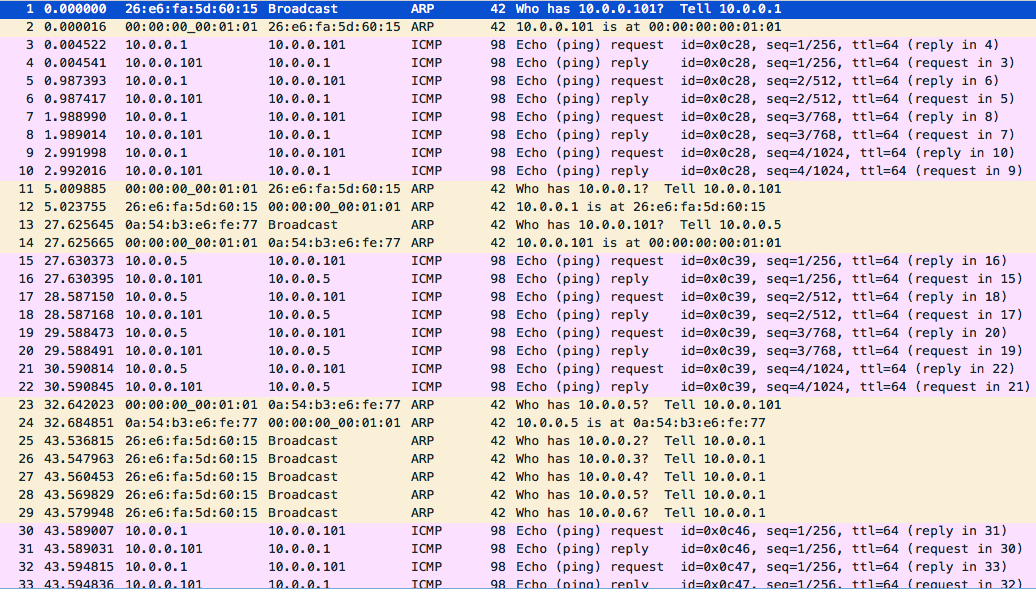
\includegraphics[scale=0.5]{images/srv1.png}
\end{center}

\hfill

En la captura de srv\_1 vemos 2 ARP seguidos de 8 PING entre 10.0.0.1 y la IP de los servidores. Corresponde al \textit{cli\_1 ping -c 4 10.0.0.101}, con el ARP request que analizará el controlador, la respuesta con MAC la del primer servidor, y 4 ping reply y 4 request con números de secuencia del 1 al 4.

A continuación, la misma situación pero con \textit{cli\_5}, pues por round-robin le correspondía el servidor 1 de nuevo, y por ello no aparecen aquí el resto de pings de los clientes.

Finalmente, una sucesión de ARP request desde el servidor al resto de clientes, pero sin respuesta, seguidos de varios mensajes PING desde y hacia los clientes 1 y 5 todos con número de secuencia 1.

Corresponde a la prueba de \textit{pingall}, donde mininet manda la orden al servidor 1 de hacer un ping a cada IP cliente, pero por los flujos en el switch, los paquetes de respuesta se reenvían a otro servidor, y como esto ocurre con cada uno de los 4 servidores, con la misma IP, se explica por qué hay 4 pares de mensajes ICMP Ping con número de secuencia siempre 1 desde cada cliente 1 y 5: por pingall, deben hacer un ping a la IP de las máquinas servidor, que tienen el mismo valor 10.0.0.101, y el switch los reenvía a la misma máquina, en este caso srv\_1.

En resumen, en pingall el servidor recibe los PING destinados a los otros servidores.

\hfill

\begin{center}
	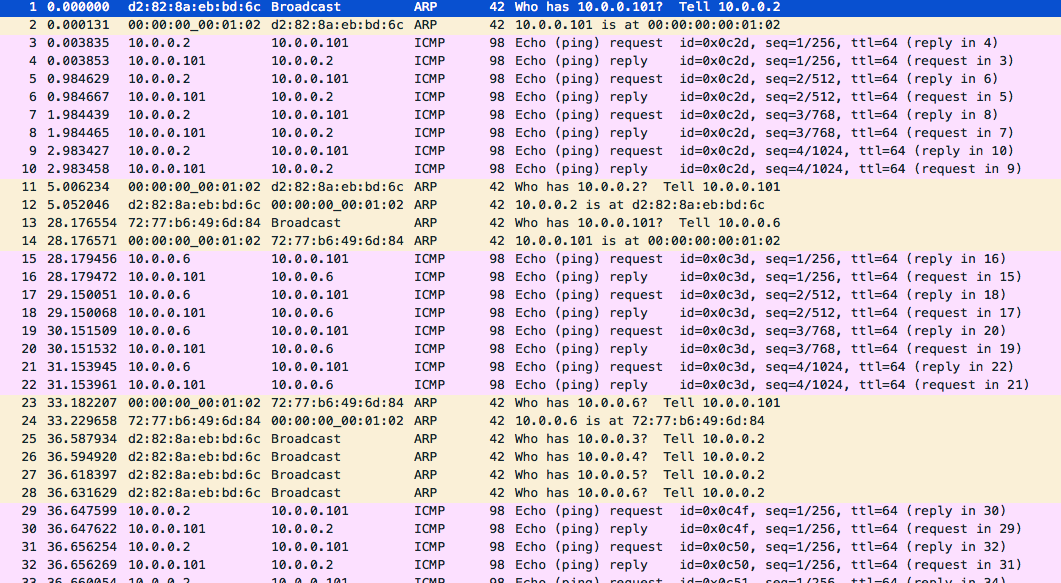
\includegraphics[scale=0.5]{images/srv2.png}
\end{center}


En el servidor 2 ocurre lo mismo que en el 1 pero con los clientes 2 y 6 que le corresponden por round-robin.

\hfill

\begin{center}
	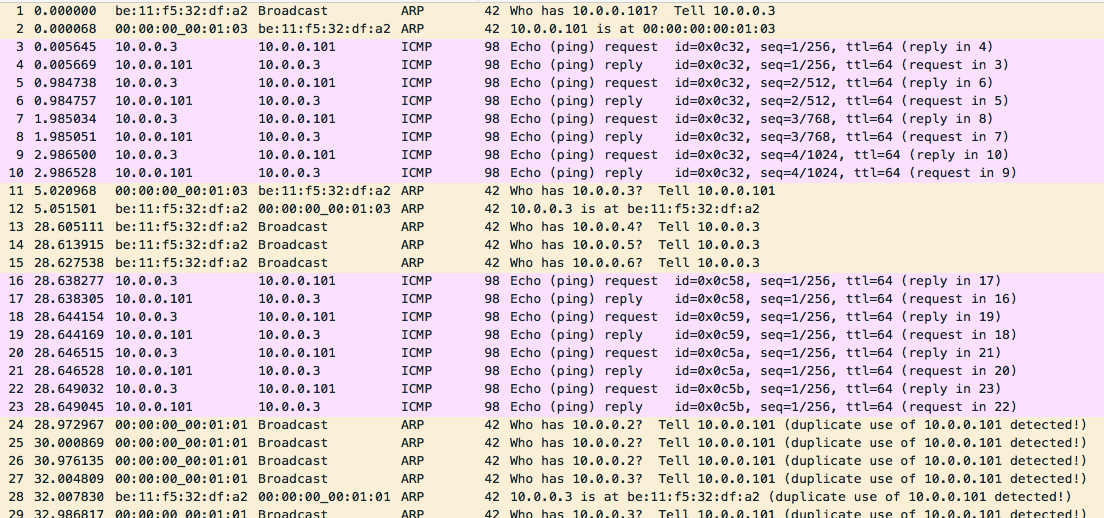
\includegraphics[scale=0.48]{images/srv3.png}
\end{center}

En el servidor 3 ocurren \textit{tres cuartos de lo mismo} que en el resto pero con sólo el cliente 3. En esta captura aprovecho para comentar lo que ocurre en los 4 servidores, pero que se ve en la imagen: wireshark detecta una IP duplicada en la red. Lo descubre porque en un ARP reply previo la IP y MAC destino eran la del servidor 3, pero el ARP request donde se detecta la duplicidad proviene de otro servidor, en la traza 24 corresponde a srv\_1, en la 39 al srv\_2, etc.

Como estos mensajes ARP request no preguntan por la IP de los servidores, se reenvían como cualquier otro paquete y no se ven afectados por los flujos que hemos programado para el balanceo.

\hfill

\begin{center}
	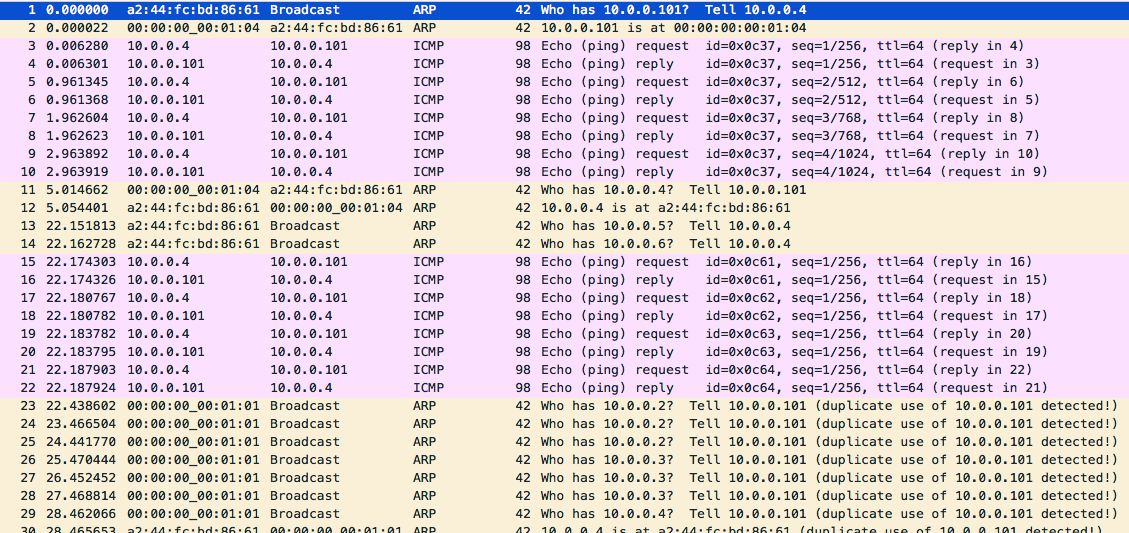
\includegraphics[scale=0.5]{images/srv4.png}
\end{center}

Y en el servidor 4 ocurre con el cliente 4 lo mismo que en el servidor 3 con el cliente 3.


\hfill


\hfill

Flujos de los switches:

\hfill

En el código del controlador de la sección anterior había comentadas dos líneas que indicaban al switch que la regla del nuevo flujo debería caducar. Para facilitar las pruebas, se comentan, y pasados unos segundos en los que las reglas de aprendizaje de macToPort sí caducan, con la orden en mininet \textit{dpctl dump-flows} se muestran las tablas con los flujos asignados por round-robin.

\hfill



\begin{Verbatim}
mininet> dpctl dump-flows
*** s1 ------------------------------------------------------------------------
NXST_FLOW reply (xid=0x4):
*** s2 ------------------------------------------------------------------------
NXST_FLOW reply (xid=0x4):
cookie=0x0, duration=390.693s, table=0, n_packets=24, n_bytes=1512, idle_age=309,
dl_src=fe:1c:e8:bb:47:2b actions=output:4
cookie=0x0, duration=397.979s, table=0, n_packets=25, n_bytes=1554, idle_age=312,
dl_src=5a:fb:3a:24:c3:d0 actions=output:3
cookie=0x0, duration=368.291s, table=0, n_packets=21, n_bytes=1386, idle_age=303,
dl_src=26:1a:ac:72:e4:51 actions=output:3
cookie=0x0, duration=383.206s, table=0, n_packets=23, n_bytes=1470, idle_age=303,
dl_src=ba:d3:b1:08:9d:20 actions=output:5
cookie=0x0, duration=406.713s, table=0, n_packets=26, n_bytes=1596, idle_age=315,
dl_src=86:bd:bc:16:52:e3 actions=output:2
cookie=0x0, duration=376.218s, table=0, n_packets=21, n_bytes=1386, idle_age=306,
dl_src=ca:6d:f2:8c:c1:a9 actions=output:2
\end{Verbatim}


Se observa que todas pertenecen a la tabla 0, y que en \textit{dl\_src} se indica la MAC de un cliente y en \textit{actions=output} el puerto por donde reenviar el paquete. Usando la información de los \textit{ifconfig} que se encuentra en el anexo, se puede hacer la correspondencia de cada cliente con su MAC y por tanto su flujo.

A los clientes 1 y 5 les corresponde el puerto 2, es decir, el servidor 1. A los clientes 2 y 6 el puerto 3, servidor 2. Al cliente 3 el puerto 4, servidor 3. Y al cliente 4 el puerto 5, servidor 4.


\hfill

Las tablas de flujos de los switchs sin que hayan caducado las entradas de macToPort son las siguientes:

\begin{Verbatim}
mininet> dpctl dump-flows
*** s1 ------------------------------------------------------------------------
NXST_FLOW reply (xid=0x4):
cookie=0x0, duration=10.672s, table=0, n_packets=3, n_bytes=126, idle_timeout=10,
 hard_timeout=30, idle_age=8, priority=65535,arp,in_port=7,vlan_tci=0x0000,
  dl_src=02:3f:e7:62:af:f1,dl_dst=00:00:00:00:01:04,arp_spa=10.0.0.6,
  arp_tpa=10.0.0.101,arp_op=2 actions=output:1
cookie=0x0, duration=8.627s, table=0, n_packets=1, n_bytes=42, idle_timeout=10,
 hard_timeout=30, idle_age=8, priority=65535,arp,in_port=5,vlan_tci=0x0000,
  dl_src=0a:27:a9:ce:34:da,dl_dst=00:00:00:00:01:04,arp_spa=10.0.0.4,
  arp_tpa=10.0.0.101,arp_op=2 actions=output:1
cookie=0x0, duration=8.666s, table=0, n_packets=1, n_bytes=42, idle_timeout=10,
 hard_timeout=30, idle_age=8, priority=65535,arp,in_port=1,vlan_tci=0x0000,
  dl_src=00:00:00:00:01:04,dl_dst=0a:27:a9:ce:34:da,arp_spa=10.0.0.101,
  arp_tpa=10.0.0.4,arp_op=1 actions=output:5
*** s2 ------------------------------------------------------------------------
NXST_FLOW reply (xid=0x4):
cookie=0x0, duration=8.673s, table=0, n_packets=1, n_bytes=42, idle_timeout=10,
 hard_timeout=30, idle_age=8, priority=65535,arp,in_port=5,vlan_tci=0x0000,
 dl_src=00:00:00:00:01:04,dl_dst=0a:27:a9:ce:34:da,
 arp_spa=10.0.0.101,arp_tpa=10.0.0.4,arp_op=1 actions=output:1
cookie=0x0, duration=117.856s, table=0, n_packets=26, n_bytes=1596, idle_age=20,
 dl_src=ba:b9:7f:25:67:db actions=output:2
cookie=0x0, duration=110.578s, table=0, n_packets=25, n_bytes=1554, idle_age=17,
 dl_src=d6:a7:d3:3c:41:ed actions=output:3
cookie=0x0, duration=78.586s, table=0, n_packets=21, n_bytes=1386, idle_age=8,
 dl_src=02:3f:e7:62:af:f1 actions=output:3
cookie=0x0, duration=86.319s, table=0, n_packets=21, n_bytes=1386, idle_age=11,
 dl_src=e6:aa:ea:b9:70:6a actions=output:2
cookie=0x0, duration=103.169s, table=0, n_packets=24, n_bytes=1512, idle_age=14,
 dl_src=f6:46:72:d8:ae:cc actions=output:4
cookie=0x0, duration=93.593s, table=0, n_packets=23, n_bytes=1470, idle_age=8,
 dl_src=0a:27:a9:ce:34:da actions=output:5
\end{Verbatim}



\section{Contribución opcional 2: 4-Balanceo complejo}

Para la mejora del balanceo complejo primero hay que definir qué tipo de tráfico se balanceará, y para eso hay que saber qué servicios ofrecerían los servidores.

En este caso supongo que entre los 4 servidores dan servicio HTTP, HTTPS y SSH, además de aceptar mensajes ICMP, que se reenviarían a servidores HTTP pues se considera que los clientes hacen ping a la web para ver si está activa.

La toma de decisiones de balanceo según el tipo de tráfico se explica a continuación en el esquema. En resumen, no todas las máquinas dan todos los servicios, y además se establecen pesos para compensar, por ejemplo, que el srv\_4 sólo ofrece SSH, mientras que srv\_2 ofrece todos.

\begin{BVerbatim}
Balanceo:
Si es ARP REQUEST a 10.0.0.101:
	Reenviar por round-robin, pero NO CREAR FLUJO, sólo reenviar.
Si es paquete IPv4:
	Si es TCP:
		Si es a puerto 80:
			Flujo a servidores 1 a 3. Pesos {1, 1, 2, 3}.
		Si es a puerto 22:
			Flujo a servidor 2 o 4. Pesos {2, 4, 4, 4, 4}
		Si es a puerto 443:
			Flujo a servidor 2 o 3. Pesos {2, 3}
	Si es UDP:
		Sólo imprimir conexión UDP.
	Si es ICMP:
		Flujo a servidores 1 a 3. Pesos {1, 1, 2, 3}.
Resto:
	"Delegar" en l2_learning
\end{BVerbatim}

En el ARP REQUEST sólo se reenvía el paquete pues no se sabe qué tipo tráfico quiere iniciar el cliente, y además puede iniciar más de uno que no vaya al mismo servidor. Por ello, se realiza un proxy con la mac de los servidores según cada tipo de flujo IP definido antes, independientemente de la dirección mac por la que pregunte el cliente.

\hfill

En el fichero \textit{balanceo.py} está todo el código del balanceador, y en este pdf explico el más representativo y no repetitivo:

Primero tenemos el balanceo con pesos. Para cada servicio un contador, un array de pesos y una función que devuelve el número del servidor (indicado dentro del array) elegido por round robin. El peso y número de servidores elegibles para el servicio se establece únicamente en el array, de modo que reajustar el balanceo es cambiar una línea de código.

\begin{lstlisting}[language=Python]
self.rrweb = 0
self.web = [1, 1, 2, 3]


def roundRobin(self):
	rr = (self.round_robin%self.max_srvs) + self.frst_prt
	self.round_robin+=1
	return rr
\end{lstlisting}


Luego tenemos un par de métodos \textit{flowToSrv} y \textit{flowToCli} casi idénticos: instalan en el switch del \textit{event} un flujo para el tipo de servicio TCP o ICMP añadiendo en las acciones la regla de cambiar la MAC del servidor (como destino u origen) por la elegida en round robin (cuando el flujo viene del cliente), o por la que el cliente preguntó (en el flujo desde el servidor), es decir, la MAC que aprendió por ARP y que se almacena en un mapa como el macToPort de l2\_learning.py.

\begin{lstlisting}[language=Python]
#Instala flujo con proxy mac del srv desde un cliente
def flowToSrv(srv, tp_port = None, ipProto = ipv4.TCP_PROTOCOL):
	print "Flujo de cli=", packet.src, " asking for ", packet.dst, " proxy a srv=", srv
	msg = of.ofp_flow_mod()
	msg.match = of.ofp_match(in_port = event.port,
								dl_src = packet.src,
								dl_dst = packet.dst,
								dl_type = 0x800, # Siempre trabajamos con IP
								nw_proto = ipProto,
								nw_src = packet.next.srcip,
								nw_dst = "10.0.0.101",
								tp_dst = tp_port)
	#msg.idle_timeout = 10
	#msg.hard_timeout = 30
	msg.actions.append(of.ofp_action_dl_addr(5, srv_to_mac[srv])) # MAC PROXY
	msg.actions.append(of.ofp_action_output(port = srv_to_port[srv]))
	msg.data = event.ofp
	self.connection.send(msg)
\end{lstlisting}

La detección del tipo de flujo, primero hay que cerciorarse de que estamos en el switch 2, y que el paquete se envía a la dirección IP de los servidores. En ese caso es un flujo desde los clientes, se debe guardar la MAC por la que pregunta y llamar a \textit{flowToSrv()}.

\begin{lstlisting}[language=Python]
# DETECCION DE FLUJOS
# Estamos en el Switch 2
if dpid_to_str(event.dpid) == "00-00-00-00-00-02":
	if packet.type == packet.IP_TYPE: # Paquete IP
		ipP = packet.next
		if ipP.dstip == "10.0.0.101" : # Se dirige a los servidores
			if ipP.protocol==ipv4.TCP_PROTOCOL: # TCP vs ICMP vs UDP
				tcpP = ipP.next
				if tcpP.dstport==80: # HTTP
					print "Conexion HTTP"
					#Calcular por round robin balanceado el 
					#servidor a reenviar el trafico
					srv = self.rr_web()
					#Guardamos por que mac preguntaba el cliente antes de aplicar proxy
					self.macToSrvWeb[packet.src] = packet.dst
					#Flujo desde el cliente al servidor aplicando proxy mac del srv
					flowToSrv(srv, tp_port=80)
					return
				elif tcpP.dstport==443: # HTTPS
				[...]
\end{lstlisting}


En caso de no ser un flujo hacia los servidores, se comprueba que sea una respuesta de ellos, de modo que se llama a \textit{flowToCli()} recuperando la MAC por la que ese cliente preguntó, y con la que hay que deshacer el proxy mac.

\begin{lstlisting}[language=Python]
[...]
elif ipP.srcip == "10.0.0.101": # Flujo de vuelta desde el servidor
	if ipP.protocol==ipv4.TCP_PROTOCOL:
		tcpP = ipP.next
		if tcpP.dstport==80: # HTTP
			print "Srv HTTP reply: srv=", packet.src
			#Paso la mac por la que pregunto el cliente, para deshacer proxy mac
			flowToCli(self.macToSrvWeb[packet.dst], tp_port = 80)
			return
		elif tcpP.dstport==443: # HTTPS
\end{lstlisting}

Finalmente, si no es un paquete IP, se comprueba que sea un ARP hacia los servidores, se aplica el mismo round robin que en la parte inicial de la práctica y sólo se reenvía el paquete, con \textit{self.connection.send(msg)}, no se crea un flujo en el switch, pues entonces no se podrían balancear los siguientes mensajes IP.

\begin{lstlisting}[language=Python]
[...]
elif ( packet.type == packet.ARP_TYPE and     # ARP REQUEST
		packet.next.opcode == arp.REQUEST and
		packet.next.protodst == "10.0.0.101" ):
	print "ARP REQUEST"
	# Round-Robin
	# Reenviar ARP, no crear flujo
	# Cualquier tipo de flujo no tenido en cuenta antes (HTTP, HTTPS, ...)
	# se reenvia por round robin a cualquier servidor
	msg = of.ofp_packet_out()
	msg.actions.append(of.ofp_action_output(port = self.roundRobin()))
	msg.data = event.ofp
	self.connection.send(msg)
	return
\end{lstlisting}








\appendix
\section{Test ping}
\begin{Verbatim}
mininet@mininet-vm:~/GitHub/mininet/scripts$ sudo ./testWcont topo.py
*** Creating network
*** Adding controller
*** Adding hosts:
cli_1 cli_2 cli_3 cli_4 cli_5 cli_6 srv_1 srv_2 srv_3 srv_4
*** Adding switches:
s1 s2
*** Adding links:
(cli_1, s1) (cli_2, s1) (cli_3, s1) (cli_4, s1) (cli_5, s1) (cli_6, s1)
 (s1, s2) (srv_1, s2) (srv_2, s2) (srv_3, s2) (srv_4, s2)
*** Configuring hosts
cli_1 cli_2 cli_3 cli_4 cli_5 cli_6 srv_1 srv_2 srv_3 srv_4
*** Starting controller
c0
*** Starting 2 switches
s1 s2 ...
*** Starting CLI:
mininet> cli_1 ping -c 4 10.0.0.101
PING 10.0.0.101 (10.0.0.101) 56(84) bytes of data.
64 bytes from 10.0.0.101: icmp_seq=1 ttl=64 time=12.2 ms
64 bytes from 10.0.0.101: icmp_seq=2 ttl=64 time=1.21 ms
64 bytes from 10.0.0.101: icmp_seq=3 ttl=64 time=0.200 ms
64 bytes from 10.0.0.101: icmp_seq=4 ttl=64 time=0.063 ms

--- 10.0.0.101 ping statistics ---
4 packets transmitted, 4 received, 0% packet loss, time 3006ms
rtt min/avg/max/mdev = 0.063/3.441/12.288/5.127 ms
mininet> cli_2 ping -c 4 10.0.0.101
PING 10.0.0.101 (10.0.0.101) 56(84) bytes of data.
64 bytes from 10.0.0.101: icmp_seq=1 ttl=64 time=31.9 ms
64 bytes from 10.0.0.101: icmp_seq=2 ttl=64 time=0.810 ms
64 bytes from 10.0.0.101: icmp_seq=3 ttl=64 time=0.071 ms
64 bytes from 10.0.0.101: icmp_seq=4 ttl=64 time=0.776 ms

--- 10.0.0.101 ping statistics ---
4 packets transmitted, 4 received, 0% packet loss, time 3000ms
rtt min/avg/max/mdev = 0.071/8.392/31.914/13.583 ms
mininet> cli_3 ping -c 4 10.0.0.101
PING 10.0.0.101 (10.0.0.101) 56(84) bytes of data.
64 bytes from 10.0.0.101: icmp_seq=1 ttl=64 time=40.4 ms
64 bytes from 10.0.0.101: icmp_seq=2 ttl=64 time=1.28 ms
64 bytes from 10.0.0.101: icmp_seq=3 ttl=64 time=0.072 ms
64 bytes from 10.0.0.101: icmp_seq=4 ttl=64 time=0.671 ms

--- 10.0.0.101 ping statistics ---
4 packets transmitted, 4 received, 0% packet loss, time 3003ms
rtt min/avg/max/mdev = 0.072/10.614/40.426/17.217 ms
mininet> cli_4 ping -c 4 10.0.0.101
PING 10.0.0.101 (10.0.0.101) 56(84) bytes of data.
64 bytes from 10.0.0.101: icmp_seq=1 ttl=64 time=28.5 ms
64 bytes from 10.0.0.101: icmp_seq=2 ttl=64 time=0.407 ms
64 bytes from 10.0.0.101: icmp_seq=3 ttl=64 time=0.073 ms
64 bytes from 10.0.0.101: icmp_seq=4 ttl=64 time=0.083 ms

--- 10.0.0.101 ping statistics ---
4 packets transmitted, 4 received, 0% packet loss, time 3004ms
rtt min/avg/max/mdev = 0.073/7.284/28.574/12.292 ms
mininet> cli_5 ping -c 4 10.0.0.101
PING 10.0.0.101 (10.0.0.101) 56(84) bytes of data.
64 bytes from 10.0.0.101: icmp_seq=1 ttl=64 time=19.3 ms
64 bytes from 10.0.0.101: icmp_seq=2 ttl=64 time=0.447 ms
64 bytes from 10.0.0.101: icmp_seq=3 ttl=64 time=0.846 ms
64 bytes from 10.0.0.101: icmp_seq=4 ttl=64 time=0.087 ms

--- 10.0.0.101 ping statistics ---
4 packets transmitted, 4 received, 0% packet loss, time 3004ms
rtt min/avg/max/mdev = 0.087/5.178/19.332/8.176 ms
mininet> cli_6 ping -c 4 10.0.0.101
PING 10.0.0.101 (10.0.0.101) 56(84) bytes of data.
64 bytes from 10.0.0.101: icmp_seq=1 ttl=64 time=38.9 ms
64 bytes from 10.0.0.101: icmp_seq=2 ttl=64 time=0.448 ms
64 bytes from 10.0.0.101: icmp_seq=3 ttl=64 time=0.597 ms
64 bytes from 10.0.0.101: icmp_seq=4 ttl=64 time=0.352 ms

--- 10.0.0.101 ping statistics ---
4 packets transmitted, 4 received, 0% packet loss, time 3006ms
rtt min/avg/max/mdev = 0.352/10.082/38.933/16.657 ms
mininet> pingall
*** Ping: testing ping reachability
cli_1 -> cli_2 cli_3 cli_4 cli_5 cli_6 srv_1 srv_2 srv_3 srv_4
cli_2 -> cli_1 cli_3 cli_4 cli_5 cli_6 srv_1 srv_2 srv_3 srv_4
cli_3 -> cli_1 cli_2 cli_4 cli_5 cli_6 srv_1 srv_2 srv_3 srv_4
cli_4 -> cli_1 cli_2 cli_3 cli_5 cli_6 srv_1 srv_2 srv_3 srv_4
cli_5 -> cli_1 cli_2 cli_3 cli_4 cli_6 srv_1 srv_2 srv_3 srv_4
cli_6 -> cli_1 cli_2 cli_3 cli_4 cli_5 srv_1 srv_2 srv_3 srv_4
srv_1 -> cli_1 X X X cli_5 X srv_2 srv_3 srv_4
srv_2 -> X cli_2 X X X cli_6 srv_1 srv_3 srv_4
srv_3 -> X X cli_3 X X X srv_1 srv_2 srv_4
srv_4 -> X X X cli_4 X X srv_1 srv_2 srv_3
*** Results: 20% dropped (72/90 received)
mininet> dpctl dump-flows
*** s1 ------------------------------------------------------------------------
NXST_FLOW reply (xid=0x4):
*** s2 ------------------------------------------------------------------------
NXST_FLOW reply (xid=0x4):
 cookie=0x0, duration=390.693s, table=0, n_packets=24, n_bytes=1512, idle_age=309,
  dl_src=fe:1c:e8:bb:47:2b actions=output:4
 cookie=0x0, duration=397.979s, table=0, n_packets=25, n_bytes=1554, idle_age=312,
  dl_src=5a:fb:3a:24:c3:d0 actions=output:3
 cookie=0x0, duration=368.291s, table=0, n_packets=21, n_bytes=1386, idle_age=303,
  dl_src=26:1a:ac:72:e4:51 actions=output:3
 cookie=0x0, duration=383.206s, table=0, n_packets=23, n_bytes=1470, idle_age=303,
  dl_src=ba:d3:b1:08:9d:20 actions=output:5
 cookie=0x0, duration=406.713s, table=0, n_packets=26, n_bytes=1596, idle_age=315,
  dl_src=86:bd:bc:16:52:e3 actions=output:2
 cookie=0x0, duration=376.218s, table=0, n_packets=21, n_bytes=1386, idle_age=306,
  dl_src=ca:6d:f2:8c:c1:a9 actions=output:2
mininet> cli_1 ifconfig
cli_1-eth0 Link encap:Ethernet  HWaddr 86:bd:bc:16:52:e3
          inet addr:10.0.0.1  Bcast:10.255.255.255  Mask:255.0.0.0
          UP BROADCAST RUNNING MULTICAST  MTU:1500  Metric:1
          RX packets:101 errors:0 dropped:0 overruns:0 frame:0
          TX packets:41 errors:0 dropped:0 overruns:0 carrier:0
          collisions:0 txqueuelen:1000
          RX bytes:5306 (5.3 KB)  TX bytes:2786 (2.7 KB)

lo        Link encap:Local Loopback
          inet addr:127.0.0.1  Mask:255.0.0.0
          UP LOOPBACK RUNNING  MTU:65536  Metric:1
          RX packets:0 errors:0 dropped:0 overruns:0 frame:0
          TX packets:0 errors:0 dropped:0 overruns:0 carrier:0
          collisions:0 txqueuelen:0
          RX bytes:0 (0.0 B)  TX bytes:0 (0.0 B)

mininet> cli_2 ifconfig
cli_2-eth0 Link encap:Ethernet  HWaddr 5a:fb:3a:24:c3:d0
          inet addr:10.0.0.2  Bcast:10.255.255.255  Mask:255.0.0.0
          UP BROADCAST RUNNING MULTICAST  MTU:1500  Metric:1
          RX packets:101 errors:0 dropped:0 overruns:0 frame:0
          TX packets:41 errors:0 dropped:0 overruns:0 carrier:0
          collisions:0 txqueuelen:1000
          RX bytes:5306 (5.3 KB)  TX bytes:2786 (2.7 KB)

lo        Link encap:Local Loopback
          inet addr:127.0.0.1  Mask:255.0.0.0
          UP LOOPBACK RUNNING  MTU:65536  Metric:1
          RX packets:0 errors:0 dropped:0 overruns:0 frame:0
          TX packets:0 errors:0 dropped:0 overruns:0 carrier:0
          collisions:0 txqueuelen:0
          RX bytes:0 (0.0 B)  TX bytes:0 (0.0 B)

mininet> cli_3 ifconfig
cli_3-eth0 Link encap:Ethernet  HWaddr fe:1c:e8:bb:47:2b
          inet addr:10.0.0.3  Bcast:10.255.255.255  Mask:255.0.0.0
          UP BROADCAST RUNNING MULTICAST  MTU:1500  Metric:1
          RX packets:101 errors:0 dropped:0 overruns:0 frame:0
          TX packets:41 errors:0 dropped:0 overruns:0 carrier:0
          collisions:0 txqueuelen:1000
          RX bytes:5306 (5.3 KB)  TX bytes:2786 (2.7 KB)

lo        Link encap:Local Loopback
          inet addr:127.0.0.1  Mask:255.0.0.0
          UP LOOPBACK RUNNING  MTU:65536  Metric:1
          RX packets:0 errors:0 dropped:0 overruns:0 frame:0
          TX packets:0 errors:0 dropped:0 overruns:0 carrier:0
          collisions:0 txqueuelen:0
          RX bytes:0 (0.0 B)  TX bytes:0 (0.0 B)

mininet> cli_4 ifconfig
cli_4-eth0 Link encap:Ethernet  HWaddr ba:d3:b1:08:9d:20
          inet addr:10.0.0.4  Bcast:10.255.255.255  Mask:255.0.0.0
          UP BROADCAST RUNNING MULTICAST  MTU:1500  Metric:1
          RX packets:101 errors:0 dropped:0 overruns:0 frame:0
          TX packets:41 errors:0 dropped:0 overruns:0 carrier:0
          collisions:0 txqueuelen:1000
          RX bytes:5306 (5.3 KB)  TX bytes:2786 (2.7 KB)

lo        Link encap:Local Loopback
          inet addr:127.0.0.1  Mask:255.0.0.0
          UP LOOPBACK RUNNING  MTU:65536  Metric:1
          RX packets:0 errors:0 dropped:0 overruns:0 frame:0
          TX packets:0 errors:0 dropped:0 overruns:0 carrier:0
          collisions:0 txqueuelen:0
          RX bytes:0 (0.0 B)  TX bytes:0 (0.0 B)

mininet> cli_5 ifconfig
cli_5-eth0 Link encap:Ethernet  HWaddr ca:6d:f2:8c:c1:a9
          inet addr:10.0.0.5  Bcast:10.255.255.255  Mask:255.0.0.0
          UP BROADCAST RUNNING MULTICAST  MTU:1500  Metric:1
          RX packets:100 errors:0 dropped:0 overruns:0 frame:0
          TX packets:40 errors:0 dropped:0 overruns:0 carrier:0
          collisions:0 txqueuelen:1000
          RX bytes:5264 (5.2 KB)  TX bytes:2744 (2.7 KB)

lo        Link encap:Local Loopback
          inet addr:127.0.0.1  Mask:255.0.0.0
          UP LOOPBACK RUNNING  MTU:65536  Metric:1
          RX packets:0 errors:0 dropped:0 overruns:0 frame:0
          TX packets:0 errors:0 dropped:0 overruns:0 carrier:0
          collisions:0 txqueuelen:0
          RX bytes:0 (0.0 B)  TX bytes:0 (0.0 B)

mininet> cli_6 ifconfig
cli_6-eth0 Link encap:Ethernet  HWaddr 26:1a:ac:72:e4:51
          inet addr:10.0.0.6  Bcast:10.255.255.255  Mask:255.0.0.0
          UP BROADCAST RUNNING MULTICAST  MTU:1500  Metric:1
          RX packets:101 errors:0 dropped:0 overruns:0 frame:0
          TX packets:41 errors:0 dropped:0 overruns:0 carrier:0
          collisions:0 txqueuelen:1000
          RX bytes:5306 (5.3 KB)  TX bytes:2786 (2.7 KB)

lo        Link encap:Local Loopback
          inet addr:127.0.0.1  Mask:255.0.0.0
          UP LOOPBACK RUNNING  MTU:65536  Metric:1
          RX packets:0 errors:0 dropped:0 overruns:0 frame:0
          TX packets:0 errors:0 dropped:0 overruns:0 carrier:0
          collisions:0 txqueuelen:0
          RX bytes:0 (0.0 B)  TX bytes:0 (0.0 B)

mininet>

\end{Verbatim}

\end{document}
